\documentclass[letterpaper,11pt]{article}

\usepackage{listings}
\usepackage{color}

\definecolor{dkgreen}{rgb}{0,0.6,0}
\definecolor{gray}{rgb}{0.5,0.5,0.5}
\definecolor{mauve}{rgb}{0.58,0,0.82}

\lstset{frame=tb,
  language=Python,
  aboveskip=3mm,
  belowskip=3mm,
  showstringspaces=false,
  columns=flexible,
  basicstyle={\small\ttfamily},
  numbers=none,
  numberstyle=\tiny\color{gray},
  keywordstyle=\color{blue},
  commentstyle=\color{dkgreen},
  stringstyle=\color{mauve},
  breaklines=true,
  breakatwhitespace=true,
  tabsize=3
}

\usepackage{setspace}
\usepackage{graphicx}
\usepackage{bm}    %for textbf
\usepackage{amsmath}
\usepackage{amsfonts}   %for mathbb
\allowdisplaybreaks[4]  %from {amsmath}
\newcommand{\independent}{\rotatebox[origin=c]{90}{$\models$}}  %from {graphicx}
\usepackage{geometry}
\geometry{letterpaper, scale=0.8}  %from {geometry}
\author{Yuan Yin}
\title{EECS 545 Homework 5}
\begin{document}\large
\maketitle
\begin{spacing}{1.2}  %from {setspace}
\section*{Problem 2) Eigenfaces}
\subsection*{a.}
The plot of sorted eigenvalues is as follows:

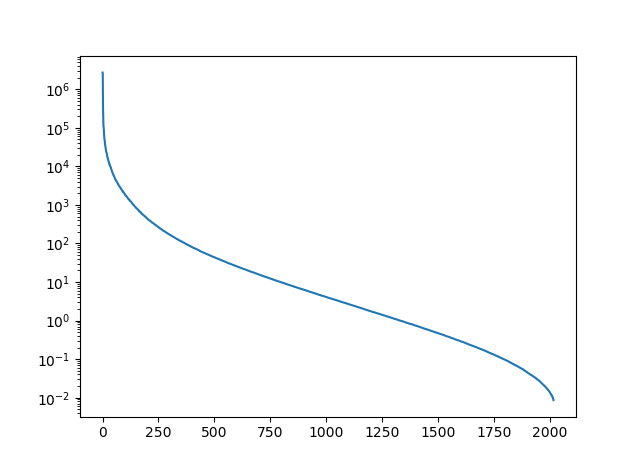
\includegraphics[width=4.95in,height=3.95in]{sorted_eigenvalues.png}

Also, the result of code is as follows:

\begin{lstlisting}
number of principal components needed to represent 95% of total variation is: 43
percentage reduction in dimension is: 97.87%
number of principal components needed to represent 99% of total variation is: 167
percentage reduction in dimension is: 91.72%
\end{lstlisting}

\subsection*{b.}
the plot of principal eigenvectors is as below:

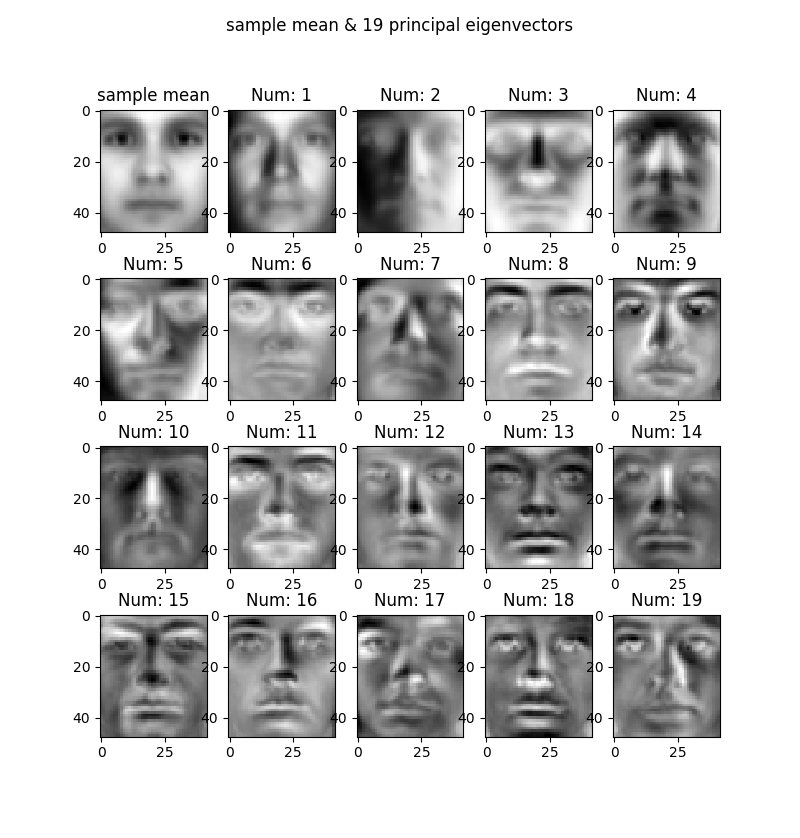
\includegraphics[width=4.95in,height=4.55in]{eigenfaces.png}

From the figure above we can find that the first 19 eigenfaces capture both facial and lighting variations. And sometimes the eigenface can capture both of them. Like the first eigenfaces, it looks like capturing the whole shape of the face. And the second captures faces with different lightness on left and right. Some of them capture the emotional expression of faces like number: 9, 13. Some of them capture both lightness and fiacial characteristics like number: 4, 8, 14, 16 and others capture only lightness of faces like number: 3, 6, 10, 11

\subsection*{c.}
The code is as follows:
\begin{lstlisting}
import numpy as np
import scipy.io as sio
import matplotlib.pyplot as plt

# Proceed with the data
yale = sio.loadmat('yalefaces.mat')
yalefaces = yale['yalefaces']
n = yalefaces.shape[2]
d = yalefaces.shape[0] * yalefaces.shape[1]
x = np.zeros([d, n])
for i in range(0, yalefaces.shape[2]):
    x[:, i] = np.reshape(yalefaces[:, :, i], d)

# Compute sample covariance matrix
mu = x.mean(axis=1)
x_bar = np.tile(mu, (n, 1)).T
s = (x - x_bar).dot((x - x_bar).T) / n

# Singular value decomposition
lamda, u = np.linalg.eig(s)
idx = lamda.argsort()[::-1]
lamda = lamda[idx]
u = u[:,idx]
plt.semilogy(lamda)
for i in range(d):
    percent = sum(lamda[:i]) / sum(lamda)
    if percent > 0.95:
        print('number of principal components needed to represent 95% of total variation is: ', i)
        print('percentage reduction in dimension is: ', '%.2f%%' % ((d - i) / d * 100))
        break
for i in range(d):
    percent = sum(lamda[:i]) / sum(lamda)
    if percent > 0.99:
        print("number of principal components needed to represent 99% of total variation is: ", i)
        print("percentage reduction in dimension is: ", '%.2f%%' % ((d - i) / d * 100))
        break

# Plot eigenvectors
fig =  plt.figure(num='eigenfaces',figsize=(8,8.5))
fig.suptitle('sample mean & 19 principal eigenvectors')
plt.subplot(4,5,1)
plt.title('sample mean')
plt.imshow(np.reshape(mu, (yalefaces.shape[0], yalefaces.shape[1])), cmap = plt.get_cmap('gray'))

for i in range(19):
    plt.subplot(4,5,2+i)
    plt.title('Num: %d' % (1 + i))
    plt.imshow(np.reshape(u[:,i], (yalefaces.shape[0], yalefaces.shape[1])), cmap = plt.get_cmap('gray'))
plt.show()
plt.close()
\end{lstlisting}

\section*{Problem 3) EM Algorithm for Mixed Linear Regression}
\subsection*{c.}
The code is as follows:
\begin{lstlisting}
import numpy as np
import matplotlib.pyplot as plt
from scipy.stats import norm
import pylab as pl

# Generating data
np.random.seed(0)
n = 200 # sample size
K = 2 # number of lines
e = np.array([0.7, 0.3]) # mixing weights
w = np.array([-2, 1]) # slopes of lines
b = np.array([0.5, -0.5]) # offsets of lines
v = np.array([0.2, 0.1]) # variances
x = np.zeros([n])
y = np.zeros([n])
for i in range(0,n):
    x[i] = np.random.rand(1)
    if np.random.rand(1) < e[0]:
        y[i] =w[0] * x[i] + b[0] + np.random.randn(1) * np.sqrt(v[0])
    else:
        y[i] = w[1] * x[i] + b[1] + np.random.randn(1) * np.sqrt(v[1])

X = np.c_[np.ones(n).T, x]
plt.plot(x, y, 'bo')
t = np.linspace(0, 1, num = 100)
plt.plot(t, w[0] * t + b[0], 'k')
plt.plot(t, w[1] * t + b[1], 'k')

# Implement EM algorithm
## Initialization
e_weight = np.array([.5, .5])
w_slope = np.array([1., -1.])
b_offset = np.array([0., 0.])
sig_var = np.array([np.var(y), np.var(y)])
iteration = 500
gamma = np.zeros([n, K])
Loglike = np.zeros(iteration)
loglike = 0
for j in range(iteration):
    new_loglike = 0
    for i in range(n):
        s = 0
        for k in range(K):
            s += e_weight[k] * norm.pdf(y[i], loc=w_slope[k] * x[i] + b_offset[k], scale=np.sqrt(sig_var[k]))
        new_loglike += np.log(s)
    ## E step
    sum = np.zeros(n)
    for i in range(n):
        sum[i] = e_weight[0] * norm.pdf(y[i], loc=w_slope[0] * x[i] + b_offset[0], scale=np.sqrt(sig_var[0])) \
                 + e_weight[1] * norm.pdf(y[i], loc=w_slope[1] * x[i] + b_offset[1], scale=np.sqrt(sig_var[1]))
        for k in range(K):
            gamma[i, k] = e_weight[k] * norm.pdf(y[i], loc=w_slope[k] * x[i] + b_offset[k], scale=np.sqrt(sig_var[k])) / sum[i]

    ## M step
    e_weight = np.sum(gamma, axis=0) / n
    for k in range(K):
        [b_offset[k], w_slope[k]] = np.asarray((np.asmatrix(X).T * np.asmatrix(np.diag(gamma[:, k])) * np.asmatrix(X)).I
                                               * np.asmatrix(X).T * np.asmatrix(np.diag(gamma[:, k])) * np.asmatrix(y).T)
        numerator = 0; denominator = 0
        for i in range(n):
            numerator += (y[i] - w_slope[k] * x[i] - b_offset[k])**2 * gamma[i, k]
            denominator += gamma[i, k]
        sig_var[k] = numerator / denominator
    if abs(new_loglike - loglike) < 10**-4:
        times = j
        break
    else:
        loglike = new_loglike
        Loglike[j] = loglike
print("The number of iterations to reach convergence is: ", times + 1)
print("The estimated model parameters are as follows: ")
print("mixing weights: ", e_weight)
print("slopes of lines: ", w_slope)
print("offsets of lines: ", b_offset)
print("variances: ", sig_var)
plt.plot(t, w_slope[0] * t + b_offset[0], '--')
plt.plot(t, w_slope[1] * t + b_offset[1], '--')

plt.figure()
iter = pl.frange(1,times)
plt.plot(iter, Loglike[:times], label = 'log-likelihood')
plt.show()
\end{lstlisting}

And the result is as follows:
\begin{lstlisting}
The number of iterations to reach convergence is: 42
The estimated model parameters are as follows: 
mixing weights:  [0.18000251 0.81999749]
slopes of lines:  [1.1010309  -1.91659525]
offsets of lines:  [-0.54270376  0.50551544]
variances:  [0.04026842 0.25301968]
\end{lstlisting}

The plot of log-likelihood as a function of iteration number is as follows:

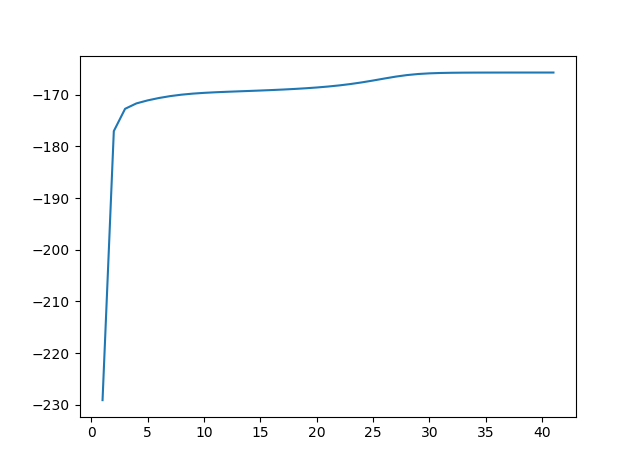
\includegraphics[width=4.95in,height=3.95in]{loglikelihood.png}

The plot of showing the data, true lines (solid) and estimated lines (dotted) is as follows:

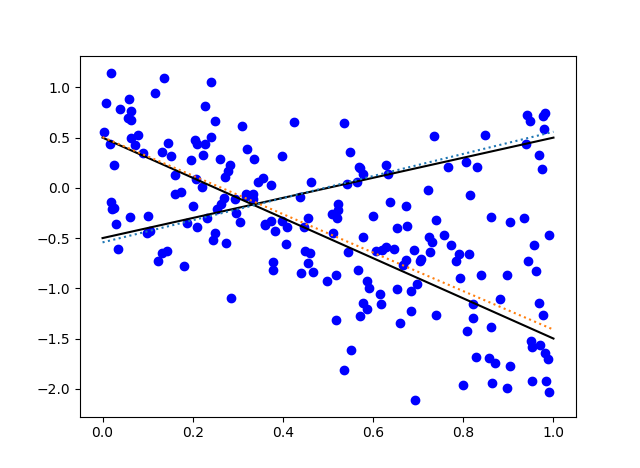
\includegraphics[width=4.95in,height=3.95in]{data_line.png}
\end{spacing}
\end{document}